[15r\textsuperscript{o}] ut hoc loco publicare velim inventum meum, cujus ope res omnis rotas concernens ad summam promoveri possit perfectionem, quod et produxi anno 1666, cum fundetur in principio capace summae perfectionis imaginabilis. Id breviter eo redit ut efficiatur compositum ex rotis dentatis, ita ut habeatur numerus dentium quantumvis, nec tamen ideo illi exigui nimis ac debiles reddantur; deinde ut motio aequaliter communicetur a rota in rotulam (+ pignon +). Tertio ut punctum contactus et sustentationis, \textit{of touching and bearing,}\edtext{}{\lemma{\textit{bearing},}\Cfootnote{a.a.O., S. 70.}} sit semper in linea duo centra jungente; \textso{quarto} ut nulla sit defrictio sive detritio: denique omnia non sunt elaborata difficiliora quam communia, excepto quod opifex his nondum assuetus. Itaque primo, si sit certus numerus requisitus dentium, 
%\begin{wrapfigure}{l}{0.5\textwidth}                    
%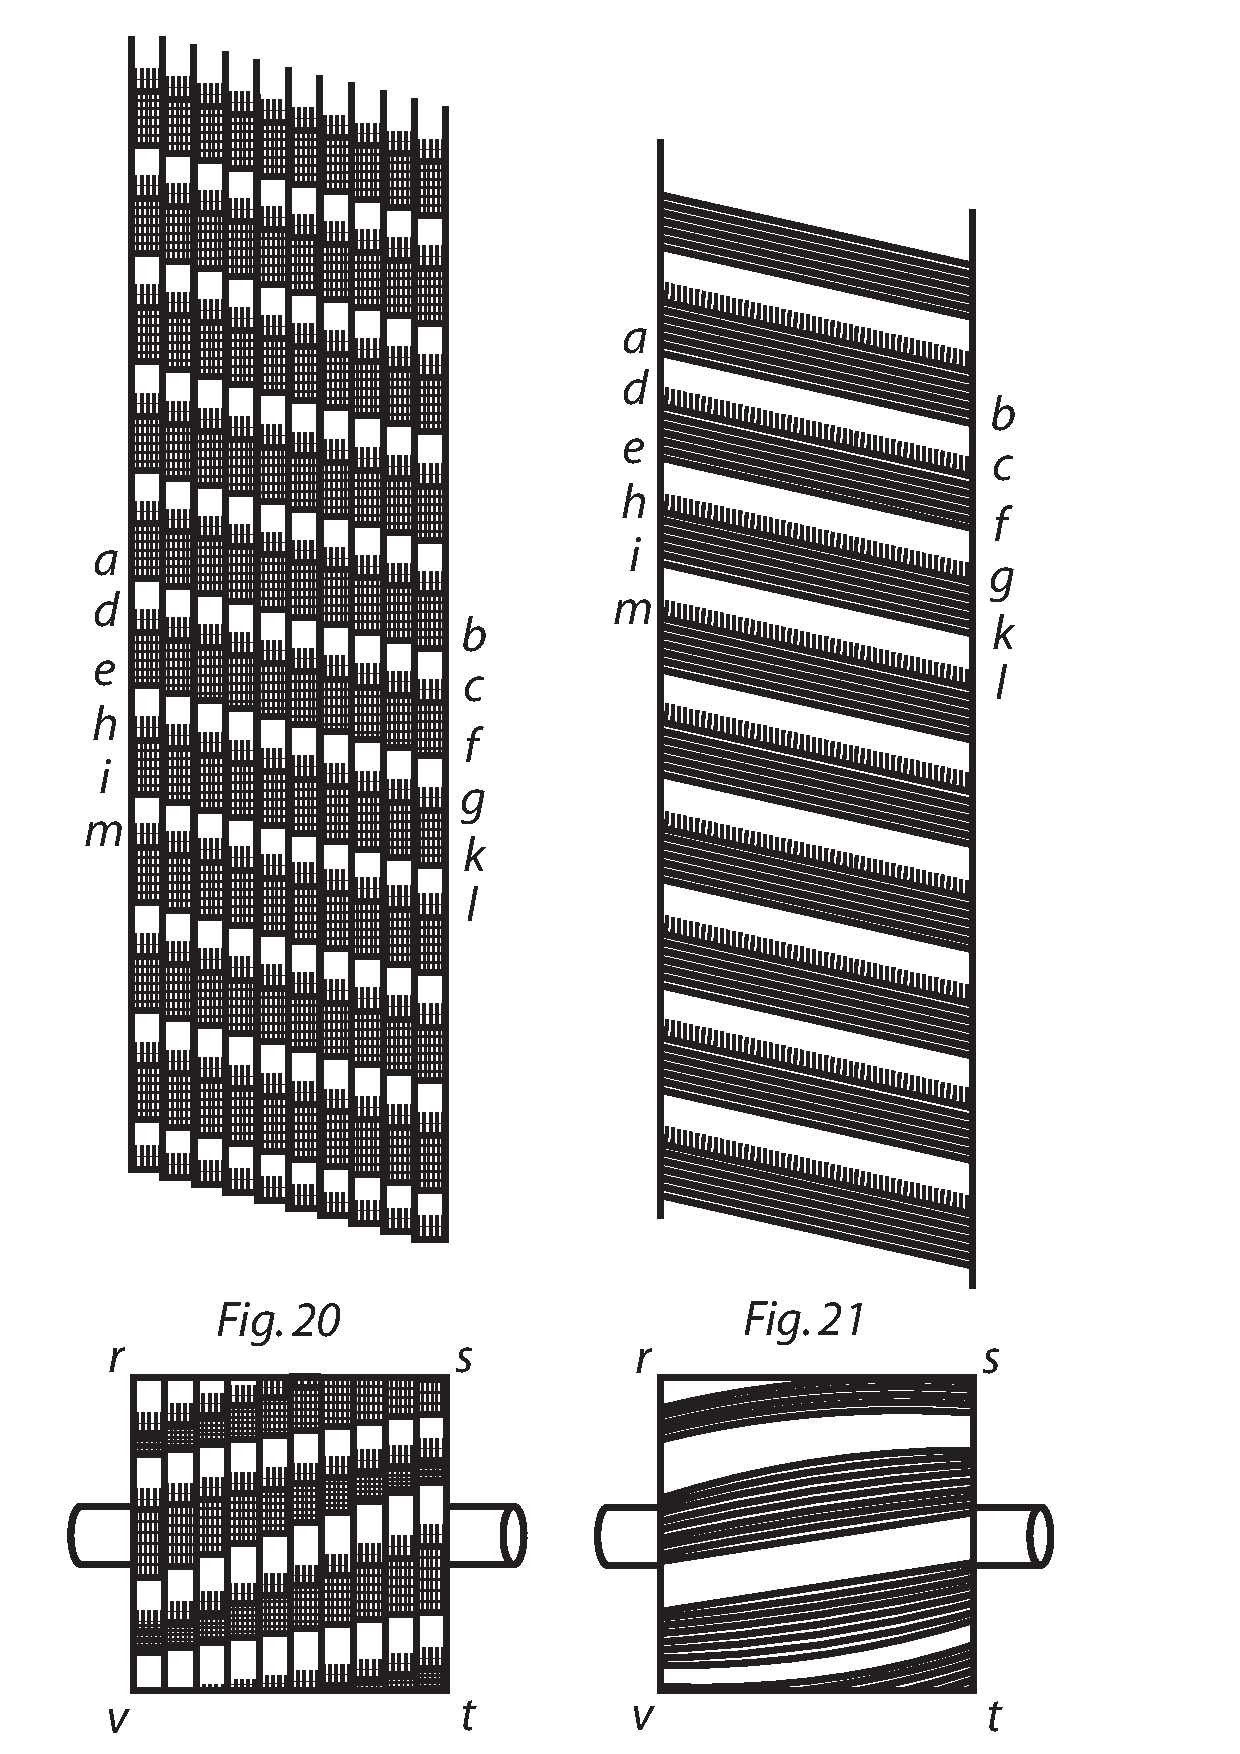
\includegraphics[width=0.5\textwidth]{images/LH0351506_014-dext20u22.pdf}\\
%\rule[0pt]{0mm}{0pt}[\textit{Fig. 9, erg. Hrsg. nach Hooke Fig. 20 u. 21}]
%\end{wrapfigure}
et non ultra requisitus faciendae exiguae rotae, necesse est, ut rotae et rotulae constent ex compluribus laminis vel rotis quae jaceant aliae apud alias, ratione quae apparet in figura 20\textsuperscript{ma}. Ibi suppone requiri ut rota habeat dentes 1000, et pignon 100, 
et dentes pariter Rotae et Rotulae (pignon) habere fortitudinem sufficientem;
\pend
\newpage
\pstart \noindent 
%\begin{wrapfigure}[27]{l}{0.52\textwidth}    
%\vspace{-6mm}                
%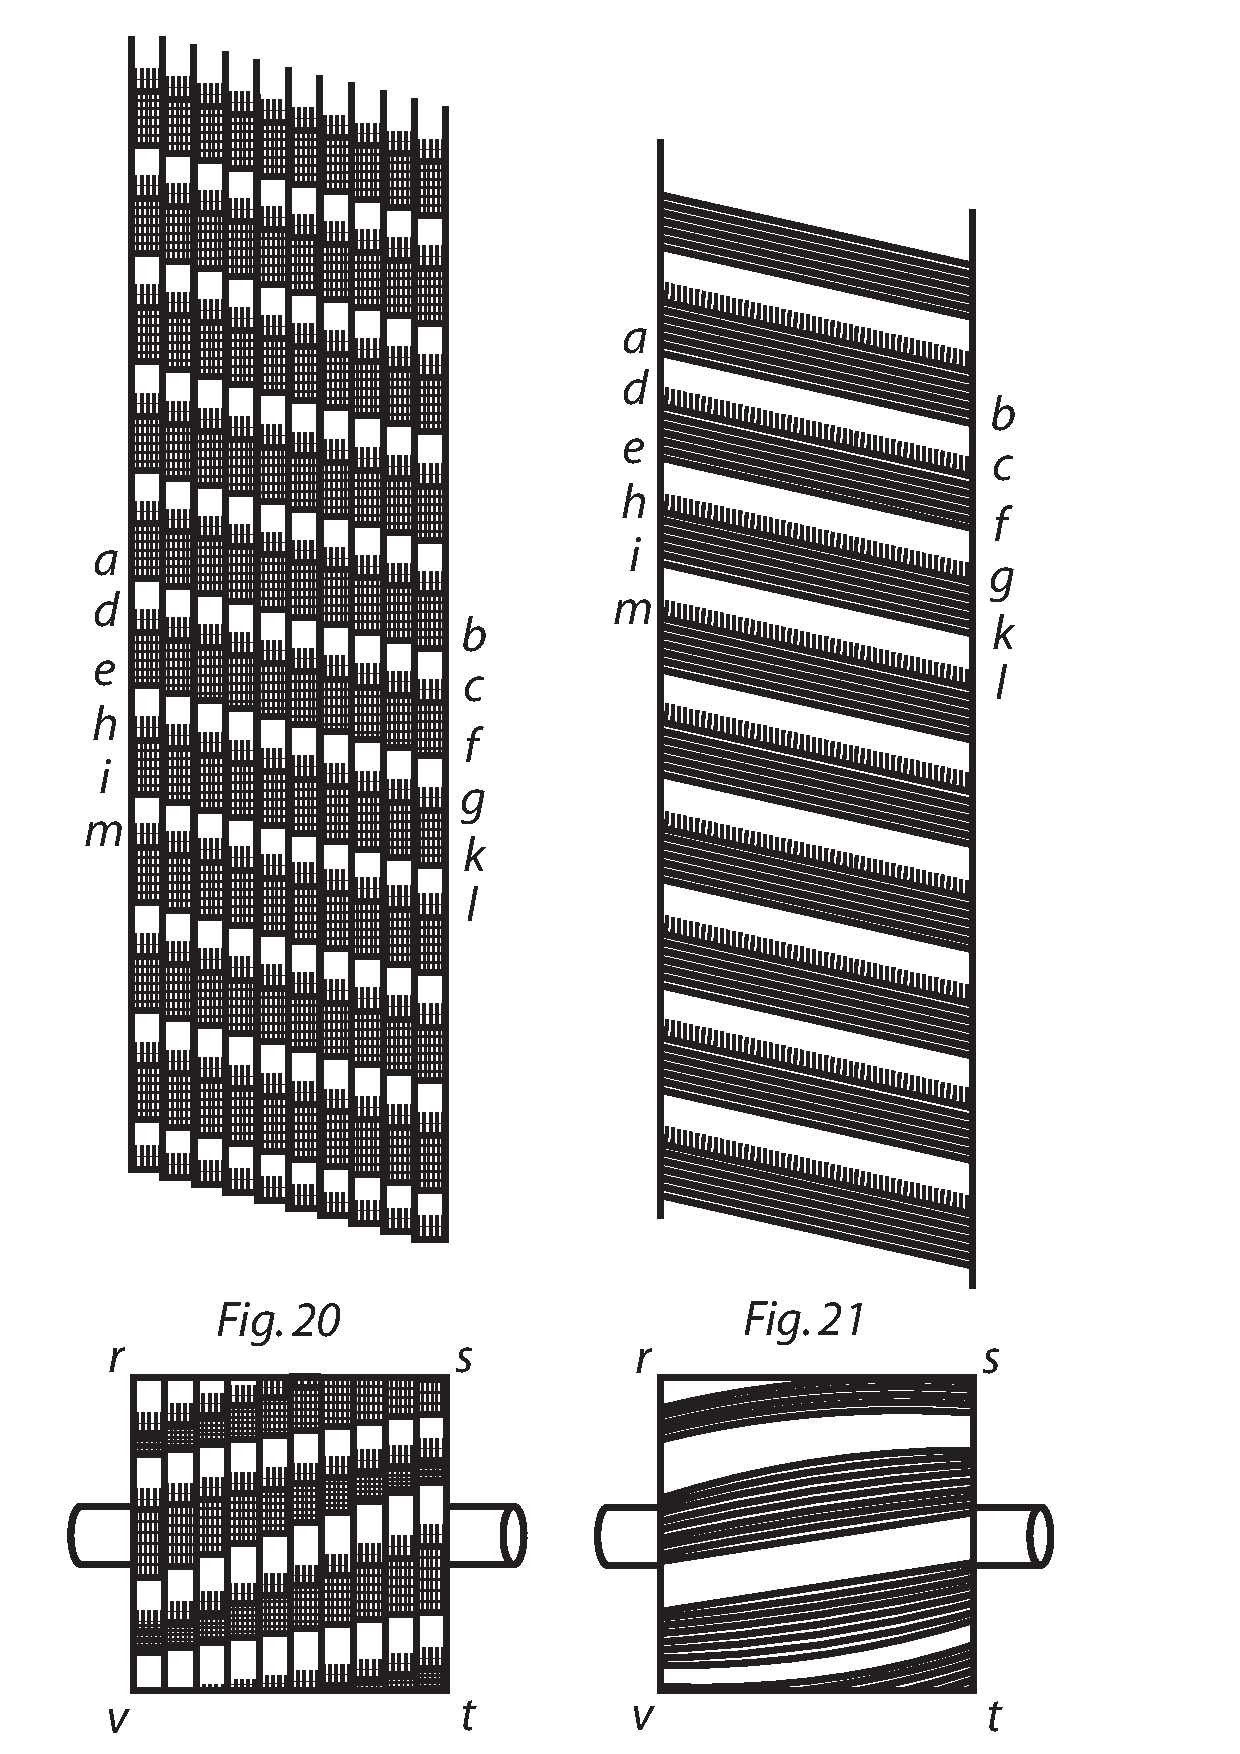
\includegraphics[trim = 0mm -2mm -5mm 0mm, clip, width=0.52\textwidth]{images/LH0351506_014-dext20u22.pdf}\\
%\rule[0pt]{0mm}{0pt}[\textit{Fig. 9, erg. Hrsg. nach Hooke Fig. 20 u. 21}]
%\end{wrapfigure}
\begin{minipage}[t]{0.52\textwidth}
\vspace{-6mm}                
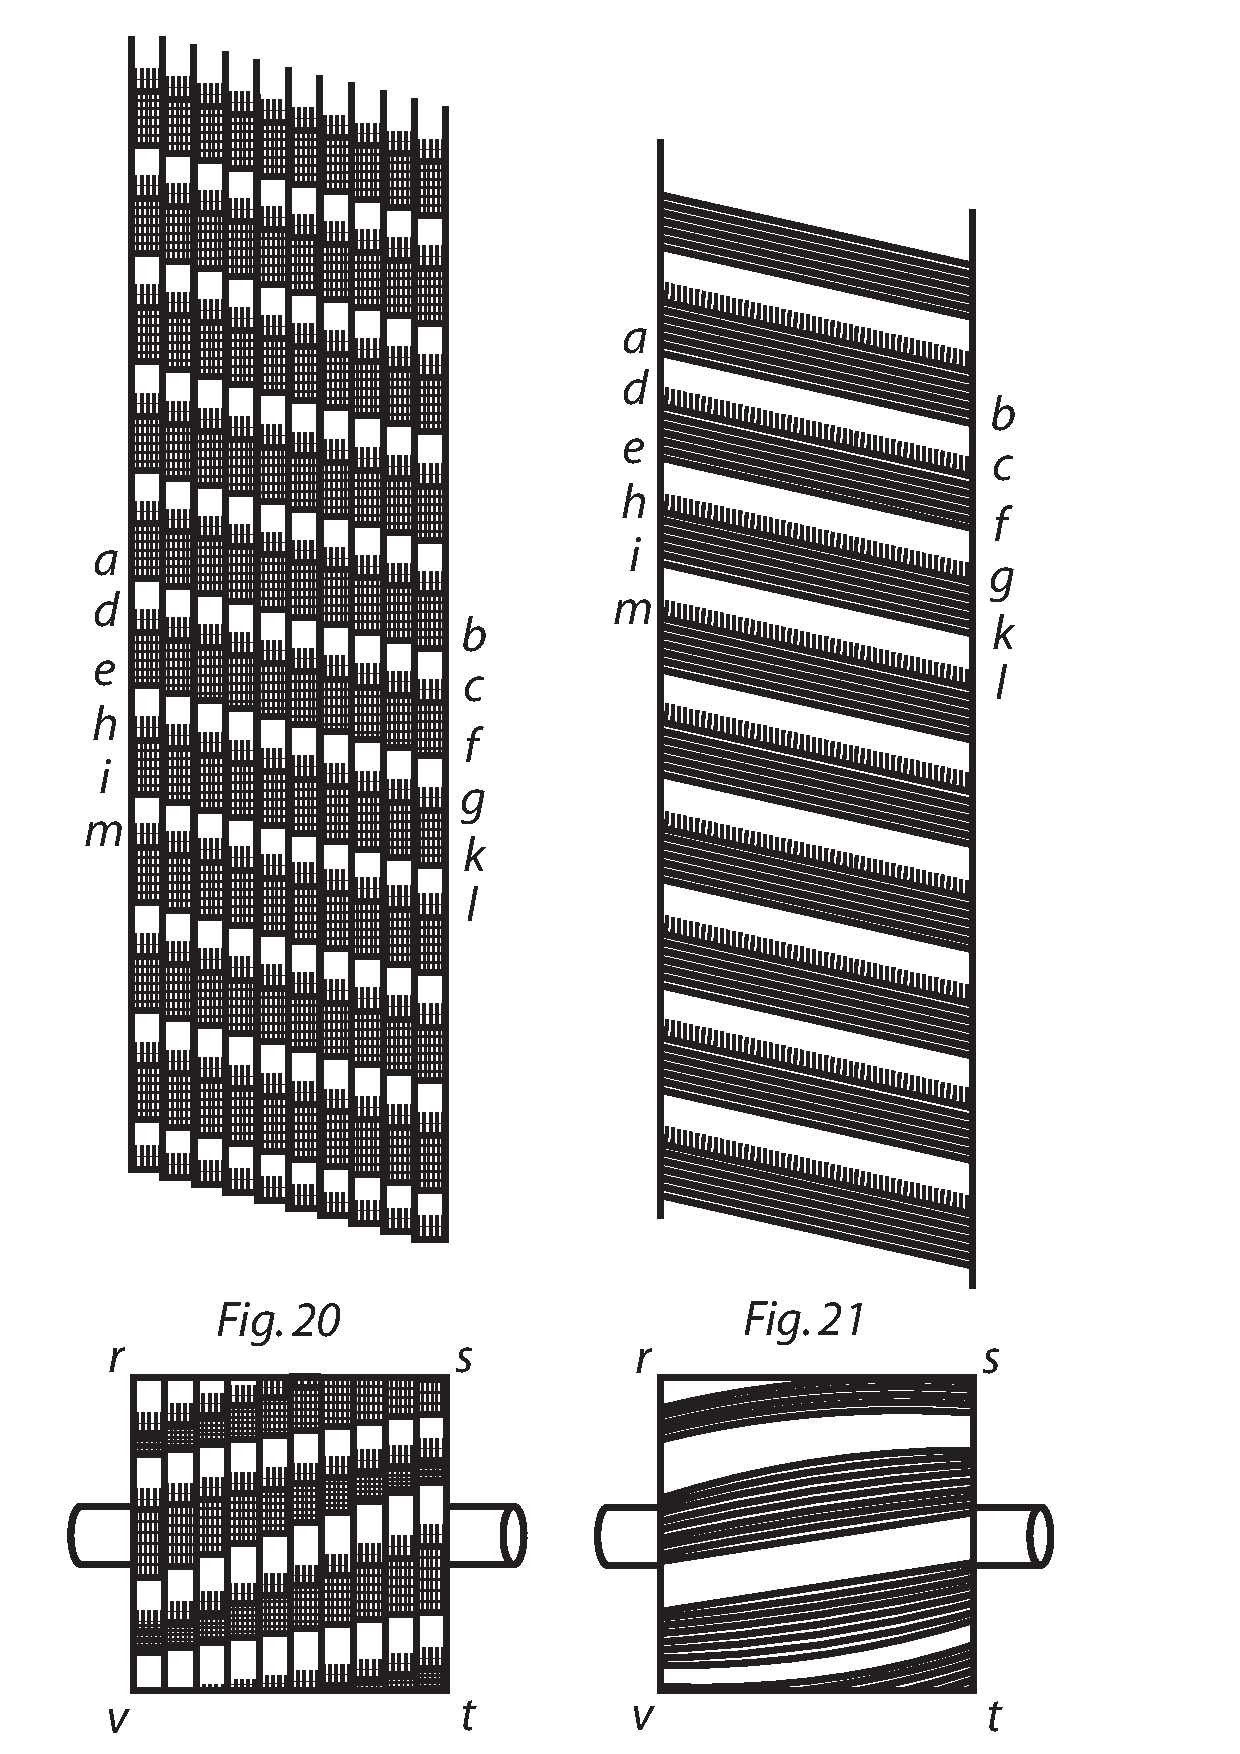
\includegraphics[width=1.0\textwidth]{images/LH0351506_014-dext20u22.pdf}\\
\rule[0pt]{0mm}{0pt}[\textit{Fig. 9, erg. Hrsg. nach Hooke Fig. 20 u. 21}]
\end{minipage}
\begin{minipage}[t]{0.4\textwidth}
sume \textit{10 Plates}\edtext{}{\lemma{\textit{10 Plates}}\Cfootnote{a.a.O., S. 71.}} (laminas) omnes ejusdem crassitiei, et ope duarum pluriumve \edtext{cochlearum firma atque contine}{\lemma{cochlearum}\Bfootnote{\textit{(1)}\ fixa \textit{(2)}\ sicut \textit{(3)}\ atque \textit{(4)}\ firma atque contine \textit{ L}}}, quasi \edtext{unam rotam;}{\lemma{}\Bfootnote{unam \textbar\ facere \textit{ gestr.}\ \textbar\ rotam; \textit{ L}}} hanc rotam seca in 100 dentes et comple; inde mediam (inter has laminas) cavitatem adapta rotundo arboris (: \textit{upon the round neck of an arbor}\edtext{}{\lemma{\textit{arbor}}\Cfootnote{a.a.O., S. 71.}} :) inde cochleam laxa, libera laminas, et eo ordine colloca, ut dentes gradualiter se sequantur, ea circiter ratione, qua expressum est in fig. 20. (: quanquam male ibi expressum propter errorem et lapsum sculptoris :) illis gradibus (\textit{steps,}\edtext{}{\lemma{\textit{steps,}}\Cfootnote{a.a.O., S. 71.}} \'{e}tages) ut ultimus dens unius gradus, proxime respondeat primo denti proximi gradus. Appello 10 dentes, \textit{comprehended within the lighter part,}\edtext{}{\lemma{\textit{part},}\Cfootnote{a.a.O., S. 71.}} \textit{abcd} vel \textit{efgh}, vel \textit{iklm}, gradum dentium \edtext{\textit{in steps;}}{\lemma{\textit{in steps;}}\Cfootnote{a.a.O., S. 71.}} et \textit{dcfe}, vel \textit{hgki}, gradum crenarum seu spatiorum \edtext{[vacuorum]}{\lemma{}\Bfootnote{vacorum \textit{\ L \"{a}ndert Hrsg.}}} interceptorum. Sed dens $bc$ [dexterrimus]\edtext{}{\Bfootnote{dexterrima \textit{\ L \"{a}ndert Hrsg.}}} debuisset locari in eodem gradu cum \textit{eh}, seu ita deprimi \edtext{ut \textit{eh}, sinisterrimo}{\lemma{ut \textit{eh},}\Bfootnote{\textit{(1)}\ et in eo \textit{(2)}\ de \textit{(3)}\ sinisterrimo \textit{L}}} seriei inferioris, quanquam lapsu sculptoris aliter hic expressum sit, unde omnis aequalitas in tangendo, ferendo, fricando in Machina Rotaria hac ratione bene elaborata, non erit major,
\end{minipage}
\pend
\pstart
\noindent
quam quae esse potest inter duos dentes proximos in uno [gradu]\edtext{}{\Bfootnote{gradum\textit{\ L \"{a}ndert Hrsg.}}}, quod est multo minus parte decima inaequalitatis quae necessario \edtext{eveniret in rota}{\lemma{}\Bfootnote{eveniret in \textbar\ in \textit{streicht Hrsg.} \textbar\ rota \textit{L}}} unius laminae 100 dentium. Secundo si desideretur, ut rota pariter et [rotula]\edtext{}{\Bfootnote{rota\textit{\ L \"{a}ndert Hrsg.}}}, habeant dentes [infinitos]\edtext{}{\Bfootnote{infinitas\textit{\ L \"{a}ndert Hrsg.}}}
omnes extremitates \edtext{}{\lemma{}\Bfootnote{extremitates \textbar\ , omnes extremitates \textit{gestr.}\ \textbar\ in \textit{L}}} in gradibus 20\textsuperscript{mae} figurae [debent]\edtext{}{\Bfootnote{debet\textit{\ L \"{a}ndert Hrsg.}}} repleri \textit{by a diagonal slope}\edtext{}{\lemma{\textit{slope}}\Cfootnote{a.a.O., S. 71.}} et [reduci]\edtext{}{\Bfootnote{reductae\textit{\ L \"{a}ndert Hrsg.}}} ad rectam, ut in fig. 21 quod nihilominus optime fiet lamina una crassitiei convenientis, cujus scilicet crassitudo sit major aut minor secundum crassitiem \textit{of the sloped thoot.}\edtext{}{\lemma{\textit{thoot}.}\Cfootnote{a.a.O., S. 71.}} Et hoc semper observandum in sectione, (quanquam aliter et falso admodum in figura expressum sit) ut extremum \textit{of one} \edtext{\textit{slope thoot}}{\lemma{\textit{slope}}\Bfootnote{\textit{(1)}\ \textit{tooth} \textit{(2)}\ \textit{thoot} \textit{L}}}\edtext{}{\lemma{\textit{slope thoot}}\Cfootnote{a.a.O., S. 71.}} ab uno latere sit \textit{full as forward as the beginning of the next toot} [\textit{on}]\edtext{}{\Bfootnote{\textit{an}\textit{\ L \"{a}ndert Hrsg.}}} \textit{the other,}\edtext{}{\lemma{\textit{other},}\Cfootnote{a.a.O., S. 71.}} hoc est extremum $bc$ unius \textit{thoot}\edtext{}{\lemma{\textit{thoot}}\Cfootnote{a.a.O., S. 71.}} (dentis an dentium ordinis) in latere recto plane sit \textit{as low as eh}\edtext{}{\lemma{\textit{as low as eh}}\Cfootnote{a.a.O., S. 71.}} initium sequentis ordinis in latere sinistro quanquam sculptoris errore hic aliter expressum sit. \edtext{Nec quicquam temporis amplius impendam}{\lemma{Nec}\Bfootnote{\textit{(1)}\ plus tempo \textit{(2)}\ quicquam temporis amplius impendam \textit{L}}} explicandis Rotulis (pignons) $rstv$, $rstv$ figurarum 20 et 21 quae sunt respondentes dentibus rotarum, tum quod res satis clara, tum quod singulari discursu plenius explicata. 